\documentclass[conference]{IEEEtran}
\usepackage{cite}
\usepackage{amsmath,amssymb,amsfonts}
\usepackage{algorithmic}
\usepackage{url}
\usepackage{graphicx}
\graphicspath{{./images/}}
\usepackage{textcomp}
\usepackage{xcolor}
\usepackage{listings}

\def\BibTeX{{\rm B\kern-.05em{\sc i\kern-.025em b}\kern-.08em
    T\kern-.1667em\lower.7ex\hbox{E}\kern-.125emX}}
\begin{document}

\title{MorteSense \\DIY Home Security}

\author{\IEEEauthorblockN{Shohin Abdulkhamidov}
      \IEEEauthorblockA{\textit{Dept. of Computer Science} \\
            \textit{San Jose State University}\\
            San Jose, United States \\
            shohin.abdulkhamidov@sjsu.edu}
      \and
      \IEEEauthorblockN{Diego Cruz}
      \IEEEauthorblockA{\textit{Dept. of Computer Science} \\
            \textit{San Jose State University}\\
            San Jose, United States \\
            diego.cruz@sjsu.edu}
      \and
      \IEEEauthorblockN{Diego Garcia-Carrasco}
      \IEEEauthorblockA{\textit{Dept. of Computer Science} \\
            \textit{San Jose State University}\\
            San Jose, United States \\
            diego.garciacarrasco@sjsu.edu}
      \and
      \IEEEauthorblockN{Spartak Gevorgyan}
      \IEEEauthorblockA{\textit{Dept. of Computer Science} \\
            \textit{San Jose State University}\\
            San Jose, United States \\
            spartak.gevorgyan@sjsu.edu}
      \and
      \IEEEauthorblockN{Faramarz Mortezaie}
      \IEEEauthorblockA{\textit{Dept. of Engineering} \\
            \textit{San Jose State University}\\
            San Jose, United States \\
            faramarz.mortezaie@sjsu.edu}

}


\maketitle

\begin{abstract}
      In recent years, DIY security system technology has been simplified. It has become cheaper for the general public.
      This includes the rise of brands focused on smart home security, such as Ring, Blink, Wyze, SimpliSafe, and Vivint,
      which offer products such as front-door cameras, infrared motion sensors/detectors, and in-home cameras
      providing different views of the house.

      One notable shortcoming of these product ecosystems is their dependence on a mobile application and a smartphone
      capable of running the application. If the application is no longer supported or the company goes out of business,
      the hardware may not function as intended, creating unnecessary e-waste and unsustainable security practices.

      This project addresses the dependence on a smartphone application by using SMS text messaging in a modular motion
      detection security system. The system will be an open ecosystem that can be tailored to the user's requirements and
      specifications and will be more sustainable, persisting even if manufacturer support is no longer available.

\end{abstract}

\begin{IEEEkeywords}
      Regular Expressions, Java, JavaScript, Kotlin, Library, Pattern Matching, Parsing
\end{IEEEkeywords}

\section{Project Overview}

\subsection{Project Goals and Objectives}
The DIY security system, more accurately described as the Microwave Motion Security System
with SMS Notifications (MMSSSN), is a project that aims to provide efficient and reliable
security for homes and businesses. The system uses microwave motion sensors to detect
movement within a certain range and sends an SMS notification to the owner's phone in
case of any suspicious activity. To manage the development process efficiently, the
team must follow the Agile Scrum framework. The user stories in this project involve
creating the sensor unit, communication module, and SMS notification system.
Project requirements include designing an intuitive user interface, ensuring
compatibility with different devices, and developing a robust and secure system that
is easy to install and operate.

\subsection{Problem and Motivation}

The Microwave Motion Security System with SMS Notifications (MMSSSN) project aims to
address the growing need for accessible, cost-effective, and reliable security solutions
for residential and commercial properties. Traditional security systems often come with high
installation and maintenance costs and complex setups, making them unattainable or
impractical for many people.

The motivation behind the MMSSSN project is to create a DIY security system that leverages
microwave motion detection technology to provide an affordable, easy-to-install, and
efficient means of monitoring and securing properties. This project is important as it will
make advanced security systems accessible to a wider audience, thus improving safety and
security for individuals and businesses.

To ensure real-time alerts, the system incorporates SMS notifications, which enable swift
responses to potential security breaches. This approach effectively addresses the need for a
more convenient and user-friendly security solution.

\subsection{Project Application and Impact}

In today's society, advanced security systems have become crucial in ensuring public health,
safety, and welfare. With growing concerns regarding security, the need for efficient and
reliable security systems is more pressing than ever. The Microwave Motion Security System
with SMS Notifications (MMSSSN) has gained popularity in recent years due to its many
benefits in preventing harm and property damage. This system has been designed with critical
factors such as global, cultural, societal, environmental, and economic considerations in
mind, ensuring accessibility and effectiveness for a wider range of users.

Public health, safety, and welfare are essential considerations for any security system.
The microwave motion security system with SMS notifications can detect and notify
homeowners of potential security risks, which is vital for public safety.
The SMS notification feature allows prompt action to be taken, reducing the risk of harm
and property damage. By reducing crime rates in a neighborhood, the security system can
also positively impact the safety and well-being of the community. In case of a security
breach, the system can notify emergency services which minimizes damage and protects lives.

\subsection{Project Results and Deliverables}

\subsubsection{Project Results}

Project results will include a microcontroller and microwave motion sensor enclosed inside
of a 3D-printed case DIY motion detector, and a deployed User Management Services (UI)
in Amazon AWS.

\subsubsection{Deliverables}

The following are the deliverables set during Spring 2023:
\begin{itemize}
      \item High-Level requirements
      \item Software Requirements Specification document
      \item Roadmap
            \subitem This involves a conversion of the provided schedule document from
            CMPE 195a into a Gantt Chart
      \item Software Backlog
            \subitem Involves documenting different product features and specifications
            according to the requirements, then assigning different people to implement them
      \item Hardware Backlog
            \subitem Involves documenting the history of making changes to the hardware,
            and figuring out the best implementations among the different configurations.
            \subitem Will mostly fall under internal-use, but will likely be occasionally
            referenced or drawn upon for project submissions
\end{itemize}

The following are the deliverables set during Summer 2023:
\begin{itemize}
      \item Creation of CAD Specification Document that will outline the
            constraints that the enclosure(s) must follow for the system
            \subitem Iterative revisions of the 3D-printed enclosure(s) will follow
            \subsubitem Likely will be logged in hardware backlog document
      \item A prototype enclosure for the central module is expected at the end of Summer 2023
\end{itemize}

The following are the deliverables set during Fall 2023:
\begin{itemize}
      \item Start of development
            \subitem Involves assembling the initial prototype of hardware and coding
            the network communication between hardware and software.
            \subitem Setting up the communication of the microcontroller and motion detector.
            \subitem The Backend API will be developed and deployed, Twilio gateway will be set up.
      \item Integration with Amazon AWS
            \subitem Integration of the User Management Service (UI) into the backend.
            \subitem Deployment and integration of Amazon AWS cloud computing,
            analytics, and reporting services.
      \item More Testing and configurations
      \item Final Deliverables
            \subitem Hardware will be enclosed in a 3D-printed case
            \subitem Final Project Presentation
\end{itemize}

\section{Background and related Work}

\subsection{Background and Technologies}

In recent years, DIY home security has risen in popularity, with modern solutions
including doorbell cameras, fingerprint-scanning door modules, infrared motion detection
sensors, and the occasional surveillance camera. Companies like Ring, Blink, Wyze,
SimpliSafe, and Vivint have had a significant impact on improving the availability of
home security and in the development of smart homes that are connected to the
Internet of Things (IoT).

Leading up to this point, contemporary literature has explored how using different parts
from different manufacturers in unique configurations can be integrated into IoT.\cite{sarhan2020}
Additionally, current literature explores how DIY home security will develop in relation
to the blockchain \cite{arifEtAl_2020} and the growing influence of machine learning.\cite{khanEtAl2021}

In light of this related work, this project entails creating a DIY security system
that will utilize contemporary microcontrollers and microwave motion detection sensors
and will be able to interface with mini-motion proximity cameras. Modular design
principles will be used to create an efficient, small-scale security system that can add
different access points through different modules. Combined with extensive documentation,
users will be able to test, maintain, and repair the system as needed.

In addition to using modular design principles, modern technologies including using Wi-Fi
to connect to remote servers and notify users of events with SMS text messaging as well
as web protocols to possibly broadcast the history of detections/captures and enact
security network management, will allow for an open ecosystem that can be tailored
to the user’s requirements/specifications and will remain sustainable by persisting
even if direct manufacturer support is no longer available.

In the context of this project, the DIY security system will build upon the work
established by research conducted by IEEE engineers and scientists that used the
Arduino platform. This project will also explore cutting-edge devices and technologies
that were not necessarily present at the time of previous studies, and further analysis
will be given in the State of the Art section following this literature review.

Komninos et al. explore the threats to smart homes and smart grids
with respect to software security and attacks involving invasions. This study uncovered
that smart grids have the threat of message modifications, replay attacks, metric
impersonation, and denial-of-service, while smart homes have similar threats, with
unique ones including false synchronization and eavesdropping.\cite{komninosEtAl2014} The main concerns
for current smart homes now include false synchronization and denial-of-service, being
the most convenient methods for burglars to effectively invade and loot a home. The two
aforementioned attacks will be of focus when developing the DIY security system, learning
from the limitations of this particular study.

A 2017 study conducted by two IEEE researchers explored the vulnerabilities that
existed in DIY home security systems that used sensors, microcontrollers,
Raspberry Pi, and ZigBee communications.\cite{joseMalekian2017} Jose and Malekian found that one limitation
of these systems at the time included the lack of an algorithm used to understand typical
user behavior and trip an alarm when the algorithm judges the detected behavior as
erratic. Another limitation of systems at the time was that the ZigBee and
IEEE 802.15.4 communications protocol were susceptible to replay attacks, allowing
attackers familiar with the technology to exploit the vulnerability and intrude into the
home.\cite{joseMalekian2017}

Arif et al. examined the development of blockchain technology and its ability to
handle great demand in its use cases. They evaluated the possibility of using blockchain
technology to back IoT devices in DIY smart home security with a proposed blockchain
configuration. They found that while it was cost-effective and remained
independent of cloud storage, the computation difficulty was set to the lowest possible,
which may become complicated as more devices are added to the security system.\cite{arifEtAl_2020}
This is a new technique gaining popularity, but further research is needed on the hardware
requirements, and it may require more resources than what had been planned for the scope
of the project. This is because the project will include web services and a deliberately
designed user experience.

IEEE member Qusay Sarhan conducted a comprehensive literature review in 2020, providing
an overview of dozens of research reports on smart home safety and security systems that
used the Arduino platform. It was found that the most significant challenges to building
these systems included physical attacks, device failure (of microcontroller/module),
power/internet outages, and software compatibility.\cite{sarhan2020} These are factors that will weigh
heavily on this project and provide a point of reference for further learning and
improving the work that has already been done in the field. Additionally, the review
provides a few subjects of interest that should be a focus for this project, including
extendability, performance, visualization, and testing for stress/robustness.\cite{sarhan2020}

Lastly, Khan et al. built on the work conducted by Arif et al. by exploring the role that
machine learning could play in home security systems that utilize blockchain technology.
They found that using a Deep Extreme Learning Machine (DELM) combined with
blockchain could prove to be far more efficient compared to other
algorithms.\cite{khanEtAl2021} Using machine learning would be beyond the scope of this project,
but it makes for an interesting way to build upon the work for a graduate research project.

\subsection{State of the Art}

The current state-of-the-art home security systems employ different techniques and
products to create a comprehensive system that can typically be tailored to the end
user through the use of modules. These products are often well-established and are only
revised in ways that are not directly observable by the end user. Rather, the underlying
technology may change while the enclosure receives minor modifications at most.\cite{sarhan2020}
The most common implementation for state-of-the-art home security systems involves the
use of modules that connect wirelessly to a central unit through some wireless protocol.\cite{joseMalekian2017}
Alternatively, each individual module can connect to the internet.\cite{sarhan2020}
From there, the modules are handled by a mobile application that allows the user to
configure notifications for detection, remotely set the alarm based on activity in
the household, or remotely activate the alarm from a safe place outside of the house
if there is dangerous activity observed within.\cite{joseMalekian2017}

Most modules are typically motion sensors or cameras, with motion sensors having had
much more development over the past few years compared to cameras. For the past
decade, motion sensors in DIY home security systems have used
Passive Infrared (PIR) technology to detect motion with changes in temperature
induced by moving objects compared to the ambient environment.\cite{sarhan2020} However, one
limitation of PIR sensors is that they cannot detect motion past objects, which
means that large furniture may prevent detection. Another limitation of PIR sensors
is that their perception of temperature may be thrown off by high ambient temperature
or by wind, meaning that if the weather is hot, it may not detect motion as a result
of a false negative, or if it is windy, it may create a false positive.\cite{sarhan2020} In short,
PIR sensors have a reduced effective distance because of the environmental factors
that can affect their ability to make accurate detections. Nonetheless, the latest
advancements have resulted in the recent acceptance of microwave motion detector
sensors that utilize the Doppler effect to detect motion behind objects and are not
susceptible to the environmental factors that impact PIR sensors.\cite{sarhan2020} This means
that cutting-edge DIY home security can more reliably detect motion behind large
furniture and can be installed outside of the house without as much concern for
environmental factors affecting the capacity to detect motion.

The Raspberry Pi and Arduino platforms have been extensively used as research tools
by the IEEE to explore different wireless communications technologies in the DIY
space, as well as for a central DIY security platform that is compared to established
home/personal security products.\cite{sarhan2020} Over the past decade, Arduinos and their
respective microcontrollers have increasingly used different connectivity types
such as XBee, Ethernet, and WiFi, most recently.\cite{sarhan2020} With the release of the
802.11n-capable Raspberry Pi Pico W in 2022, the project anticipates building
upon the work covered by previous research that used both mainline platforms or
similar microcontrollers.

\section{System Design}

\subsection{Architecture Design}

\subsubsection{Project Hardware Architecture}

\begin{figure}[htbp]
      \centering
      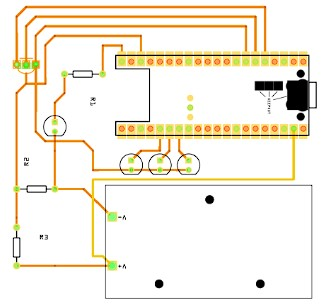
\includegraphics[width=0.8\linewidth]{pcbDiagram.jpg}
      \caption{PCB Diagram}
      \label{fig:pcbDiagram}
\end{figure}

The PCB (Printed Circuit Board Diagram) diagram depicts the layout of the DIY security
circuit board. It shows the placement of components and their interconnections on the
board, as well as any necessary information related to the fabrication and assembly of
the board. While a circuit diagram provides a schematic representation of the electrical
connections between components, the PCB diagram shows the physical layout of the
components and the soldering points between them and the soldering layers. It is
important for the efficient routing of traces and connections and will be used during
the fabrication process.

The PCB will have 3 main components, the Raspberry Pi Pico W Microcontroller with
2.4Ghz Wi-Fi Module which is in the right top corner, the 9V Battery input in the
right bottom corner, and finally, it will have the 5.8Ghz Microwave Motion Sensor
which is in the left top corner of the board. The motion sensor emits electromagnetic
waves which are then reflected back to the receiver and analyzed. If the waves are
altered that means the object that reflected them is moving. The board also will have
4 LED indicators for showing the WI-FI connection indicator, power indicator,
motion detection indicator, and connection to backend service indicator.
Rx-Tx serial communication will be used between the microcontroller and motion sensor,
for all other communication GP pins will be used.

The hardware has two main components, the motion detector, and the microcontroller.
The microcontroller uses Rx-Tx serial communication to send and receive information
into the motion detector in the form of bits, which can be used to send and receive
instructions. Microwave Sensor out signal is used to detect the motion itself.
As the microcontroller comes with an integrated Wi-Fi module, it will be used to
communicate with the backend by sending and receiving API requests.
The device will enter sleep mode and only be activated during motion detection,
this will allow us to lower the power consumption significantly.
All the hardware will be programmed in C and Micropython.

The microcontroller has an integrated server with web UI, which allows users
to connect to it with their home devices such as smartphones, and do an easy setup
of the systems, such as the Wi-Fi module. UI also provides basic information regarding
the status of the motion detection device, battery lifetime, and other necessary
information. The microcontroller has full control over the motion detector which
allows users to do the precise configuration of system parameters, such as motion
detection range, sensitivity, etc.

\begin{figure}[htbp]
      \centering
      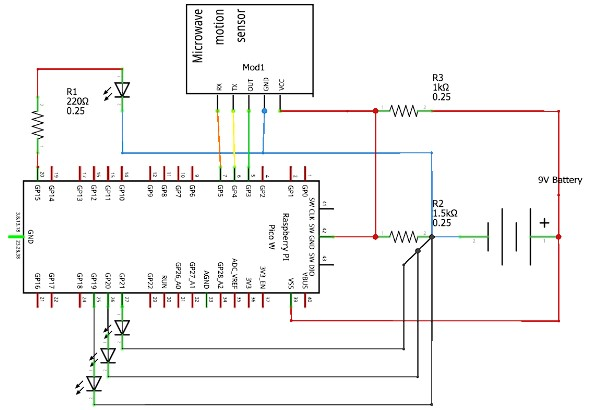
\includegraphics[width=0.8\linewidth]{hardwareArchitecture.jpg}
      \caption{Project Hardware Architecture}
      \label{fig:hardwareArchitecture}
\end{figure}

\subsubsection{Project Software Architecture}

The Notification Service is responsible for processing and sending SMS notifications
to users when the motion is detected. It receives the motion detection information
through requests from sensor management software and sends SMS notifications to the
registered mobile numbers. Notification Service will integrate SMS gateway using
Twilio API for communication with Client Devices. A database is required to store
information about the user systems, such as user information, sensor information,
and notification settings. The Reporting and Analytics component is responsible
for generating reports on the system’s performance, such as the number of motion
detections per day and average response time. It will help to analyze and further
improve the quality of the systems.

\begin{figure}[htbp]
      \centering
      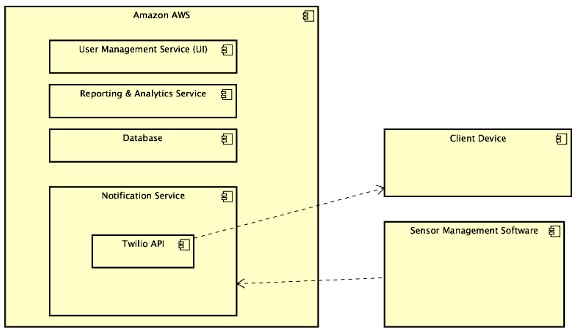
\includegraphics[width=0.8\linewidth]{softwareArchitecture}
      \caption{Software Architecture}
      \label{fig:softwareArchitecture}
\end{figure}

User Management Service (UI) will provide an interface for users to register and
authenticate their devices and configure notification settings. It will provide an
event log, which allows users to manage events related to sensors. Additionally, it
will have an audit trail of all activity in the system, including user activity.
The systems above will be powered by Amazon AWS, it allows us to expand and process
the volume of traffic.

\begin{figure}[htbp]
      \centering
      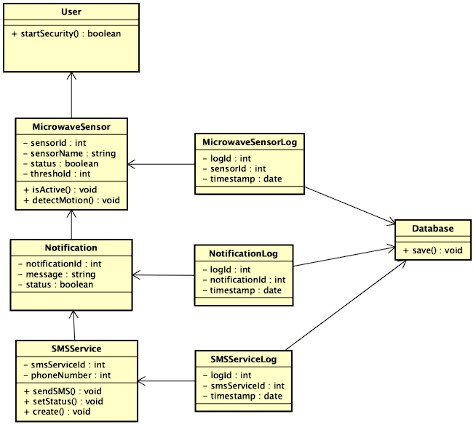
\includegraphics[width=0.8\linewidth]{softwareClassDiagram.jpg}
      \caption{Software Class Diagram}
      \label{fig:softwareClassDiagram}
\end{figure}

The Class Diagram represents the relationships between various classes in the
Microwave Motion Security System with SMS Notifications. The User class is associated
with the MicrowaveSensor class, which is responsible for detecting motion.
The SMSService class is associated with the Database class, which is used to store
data related to the SMS services used to send SMS messages to the user.
The MicrowaveSensor class is associated with the Notification and SMSService classes,
which are responsible for sending notifications and SMS messages to the user when
motion is detected. These associations enable the MicrowaveSensor to trigger the
Notification and SMSService classes to send a notification and an SMS message
to the user, respectively.

The Database class is associated with the Notification, NotificationLog, SMSService,
SMSServiceLog, and SensorLog classes, which are used to store data related to
notifications, SMS services, and sensor logs. The Notification and SMSService
classes have a one-way association with the Database class, indicating that they
can use the Database to store data related to the notifications and SMS services
sent to the user. Additionally, the Notification and SMSService classes have
composition relationships with the NotificationLog and SMSServiceLog classes, respectively.
These composition relationships indicate that a Notification or a SMSService "has-a"
relationship with their respective log tables, and the log tables cannot exist
independently of the Notification or SMSService.

Finally, the SensorLog class has a one-way association with the MicrowaveSensor class,
which indicates that it can store data related to the logs of the microwave sensors
used for detecting motion. Overall, the Class Diagram demonstrates the flow of
information and data between the various classes and tables in the system, providing a
comprehensive representation of the Microwave Motion Security System with
SMS Notifications.

\begin{figure}[htbp]
      \centering
      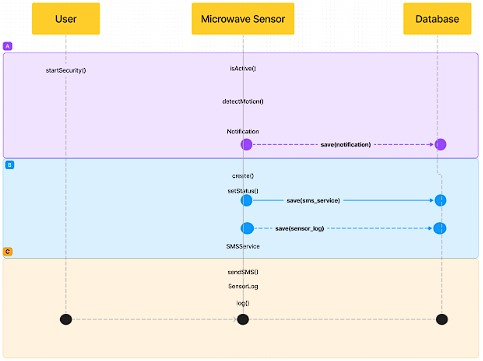
\includegraphics[width=0.8\linewidth]{softwareSeqDiagram.jpg}
      \caption{Software Sequence Diagram}
      \label{fig:softwareSeqDiagram}
\end{figure}

The sequence of events is as follows:
\begin{enumerate}
      \item The User triggers the Microwave Sensor to start monitoring for motion detection
            by calling the startSecurity() method.
      \item The MicrowaveSensor detects motion and triggers the Notification and SMSService
            to send a notification and an SMS message to the user, respectively.
      \item The Notification creates a new notification by calling the create() method,
            which generates a new notification ID.
      \item The Notification saves the notification data to the Database by calling the
            save(notification) method.
      \item The Notification sets the status of the notification to "sent" by calling the
            setStatus("sent") method.
      \item The SMSService creates a new SMS service by calling the create() method,
            which generates a new smsServiceId.
      \item The SMSService saves the SMS service data to the Database by calling the
            save(sms\_service) method.
      \item The SMSService sets the status of the SMS service to "sent" by calling the
            setStatus("sent") method.
      \item The SMSService sends an SMS message to the user by calling the sendSMS() method.
      \item The SMSService saves the log data related to the SMS message to the
            SMSServiceLog table by calling the save(sms\_service\_log) method.
      \item The Notification saves the log data related to the notification to the
            NotificationLog table by calling the save(notification\_log) method.
\end{enumerate}

In this way, the system can detect motion using the MicrowaveSensor, send notifications
and SMS messages to the user using the Notification and SMSService classes, respectively,
and store data related to these events using the Database, NotificationLog, and
SMSServiceLog tables.

\subsection{Design Constraints, Problems, Trade-offs, and Solutions}

\subsubsection{Design Constraints and Challenges}

Designing a DIY home security system presents several constraints and challenges that
require careful consideration. The primary requirement for the system is that it should
be easy to use, install, and work seamlessly across a diverse range of devices, which
necessitates careful consideration of the user interface and communication protocols.
Additionally, the system must be robust and secure to ensure that it is not easily
hacked or compromised. This requires implementing encryption and secure data storage
methods. Furthermore, the system should have low power consumption, which necessitates
the use of sleep modes and energy-efficient components.

Lastly, the design must account for trade-offs, such as balancing the range and
sensitivity of the motion sensor with the overall system cost and size. For example,
the dimensions of the hardware enclosure should facilitate mounting the module on the
doorstep or on the wall at an angle that can provide a coverage angle between a
typical visual coverage range of 60 to 75 degrees. However, the dimensions of the
hardware enclosure should not be too tall or too wide, as it may cause unequal weight
distribution after mounting the enclosure.

\subsubsection{Design Solutions and Trade-offs}

An alternative design being explored is to use a different power source,
such as a higher-voltage battery or a lower-voltage C/D battery, compared to the
current 9V design. However, using a lower voltage battery like AA/AAA would result
in less effective mAh and shorter battery life for the system. When using batteries
like C/D, another challenge is the additional space it would require in the enclosure,
making it heavier and more difficult to mount on walls or ceilings. For this project,
9V batteries offer the best compromise, as they have a reasonable form factor in the
shape of a rectangular enclosure with rounded edges, making it easy to design a
3D-printed enclosure with the help of CAD software.

To address the constraints and challenges of designing a DIY home security system,
several solutions and trade-offs have been incorporated into the system. The user
interface design aims to make it intuitive and user-friendly for users with different
technical proficiency levels. Compatibility is achieved by using widely adopted
communication protocols and a microcontroller with an integrated Wi-Fi module.
To ensure robust security, the system employs contemporary encryption techniques
and secure data storage methods, including a secure database hosted on Amazon AWS.
In terms of energy efficiency, the device enters sleep mode when not actively
detecting motion, reducing power consumption. The system also includes trade-offs,
such as optimizing the motion sensor's range and sensitivity, which may impact the
overall cost and size of the system. Ultimately, these design solutions and
trade-offs contribute to a balanced, effective DIY home security system.

\bibliographystyle{IEEEtran}
\bibliography{MorteSense}

\end{document}